% ===================================================================
% Method diagram for the EEG-to-image paper (NeurIPS 2026 submission).
% Mirrors the 3-stage layout of the reference figure
% (inputs/figures/method_thought_text (1).jpg) but adapts it to our two
% pipelines that share a single frozen frontend.
%
% Compile (any of the following):
%   pdflatex method_diagram.tex
%   latexmk -pdf method_diagram.tex
%
% Output: method_diagram.pdf  (tightly cropped, vector graphics).
% Include in main_v3.tex with:
%   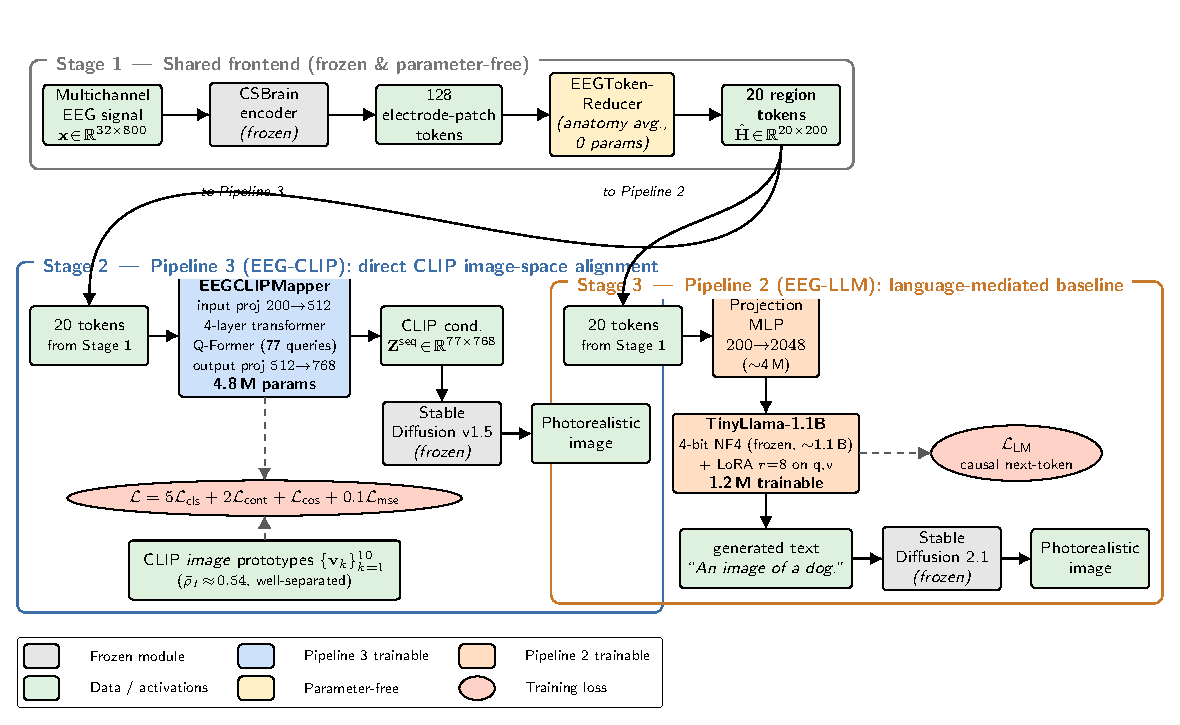
\includegraphics[width=\linewidth]{method_diagram.pdf}
% ===================================================================

\documentclass[border=8pt]{standalone}

\usepackage{tikz}
\usepackage{amsmath}
\usepackage{amssymb}
\usetikzlibrary{positioning, arrows.meta, shapes.geometric, fit, backgrounds, calc}

% ---------- colours (muted, paper-safe) ----------
\definecolor{frozenC}{RGB}{230,230,230}     % grey   = frozen
\definecolor{trainP3}{RGB}{205,225,250}     % blue   = Pipeline 3 trainable
\definecolor{trainP2}{RGB}{255,222,196}     % orange = Pipeline 2 trainable
\definecolor{dataC}{RGB}{222,240,222}       % green  = data / activations
\definecolor{anatC}{RGB}{255,240,200}       % yellow = parameter-free op
\definecolor{lossC}{RGB}{255,210,200}       % red    = loss
\definecolor{panelP1}{RGB}{120,120,120}
\definecolor{panelP3}{RGB}{60,110,170}
\definecolor{panelP2}{RGB}{200,120,40}

\begin{document}
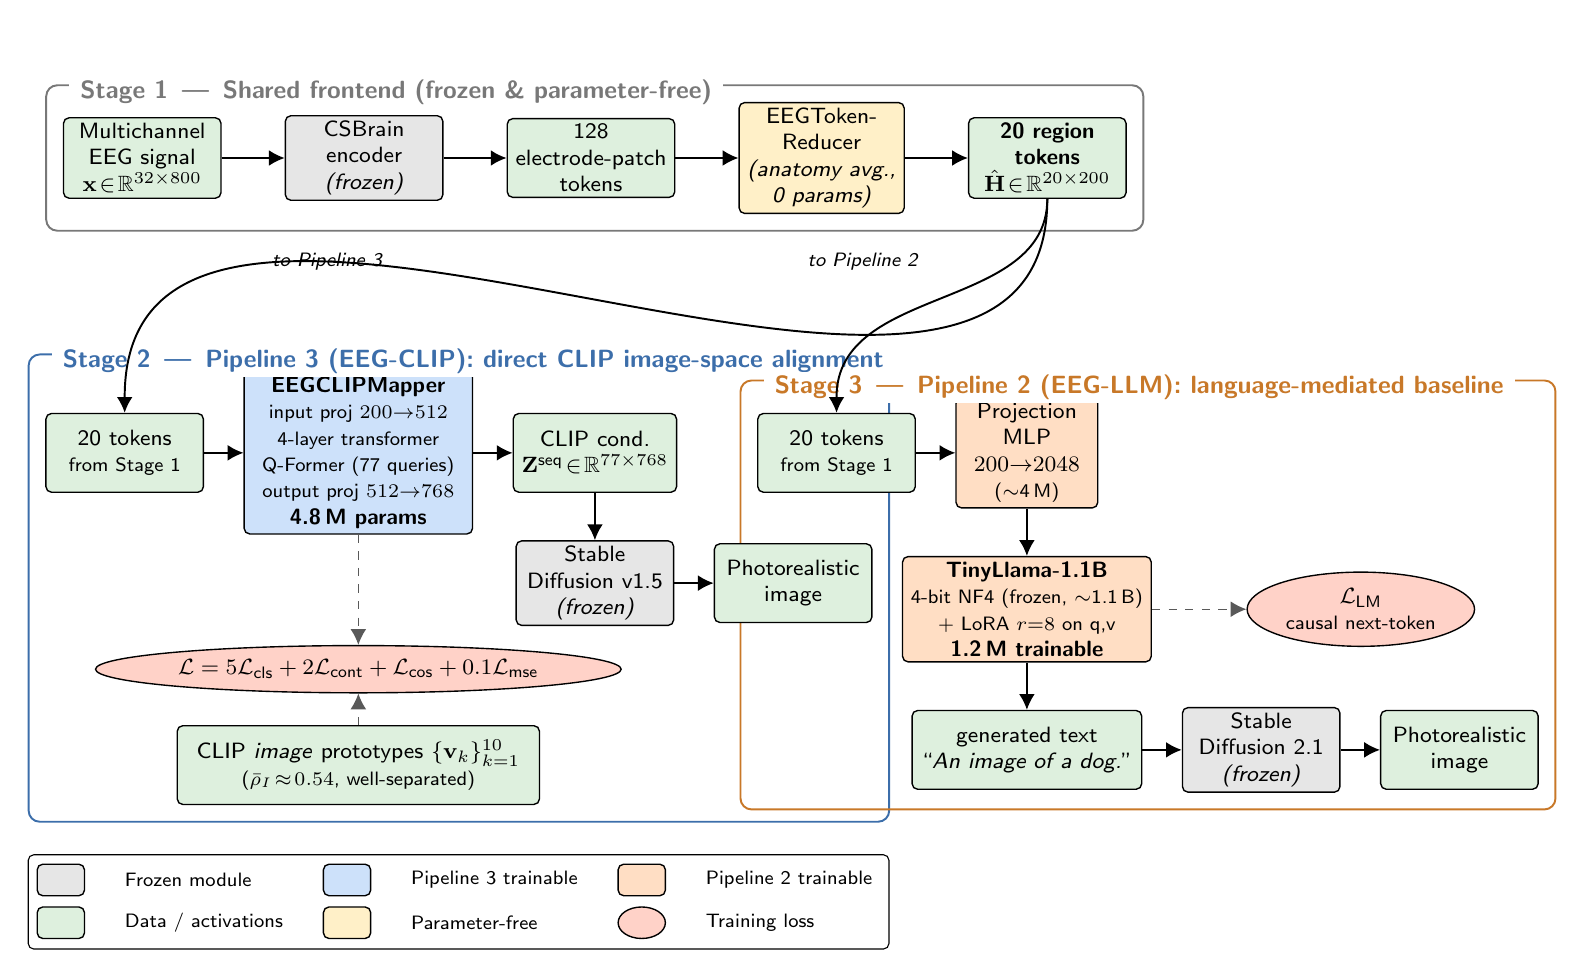
\begin{tikzpicture}[
  font=\sffamily\footnotesize,
  >={Latex[length=2mm,width=2mm]},
  thick,
  block/.style={
    draw, rounded corners=2pt, align=center,
    minimum height=10mm, minimum width=20mm,
    inner xsep=3pt, inner ysep=2pt, line width=0.5pt
  },
  frozen/.style ={block, fill=frozenC},
  pthree/.style ={block, fill=trainP3},
  ptwo/.style   ={block, fill=trainP2},
  dat/.style    ={block, fill=dataC},
  anat/.style   ={block, fill=anatC},
  loss/.style   ={ellipse, draw, fill=lossC, align=center,
                  inner sep=2pt, line width=0.5pt, minimum height=6mm},
  arr/.style    ={->, line width=0.6pt},
  arrdash/.style={->, line width=0.5pt, dashed, gray!70!black},
  panel/.style  ={draw, rounded corners=4pt, line width=0.7pt, inner sep=6pt},
  paneltitle/.style={fill=white, inner xsep=4pt, inner ysep=1pt,
                     font=\sffamily\bfseries\small}
]

% ====================================================================
%                STAGE 1  --  shared frozen frontend
% ====================================================================

\node[dat]                              (eeg)   at (0,0)
  {Multichannel\\EEG signal\\$\mathbf{x}\!\in\!\mathbb{R}^{32\times 800}$};
\node[frozen, right=8mm of eeg]         (csb)
  {CSBrain\\encoder\\\textit{(frozen)}};
\node[dat,    right=8mm of csb]         (h128)
  {128\\electrode-patch\\tokens};
\node[anat,   right=8mm of h128]        (red)
  {EEGToken-\\Reducer\\\textit{(anatomy avg.,}\\\textit{0 params)}};
\node[dat,    right=8mm of red]         (h20)
  {\textbf{20 region}\\\textbf{tokens}\\$\hat{\mathbf{H}}\!\in\!\mathbb{R}^{20\times 200}$};

\draw[arr] (eeg) -- (csb);
\draw[arr] (csb) -- (h128);
\draw[arr] (h128) -- (red);
\draw[arr] (red) -- (h20);

\begin{pgfonlayer}{background}
\node[panel, draw=panelP1, fit=(eeg)(csb)(h128)(red)(h20)] (s1) {};
\end{pgfonlayer}
\node[paneltitle, anchor=north west, text=panelP1] at ($(s1.north west)+(3mm,1mm)$)
  {Stage 1 \,---\, Shared frontend (frozen \& parameter-free)};

% Two routing arrows out of stage 1 down to the two pipelines
\coordinate (h20bot) at ($(h20.south)+(0,0)$);
\node[font=\sffamily\itshape\scriptsize, anchor=north]
   at ($(s1.south)+(-3.4cm,-1.5mm)$) {to Pipeline 3};
\node[font=\sffamily\itshape\scriptsize, anchor=north]
   at ($(s1.south)+(3.4cm,-1.5mm)$)  {to Pipeline 2};


% ====================================================================
%       STAGE 2  --  Pipeline 3 (EEG-CLIP)         (bottom-left)
% ====================================================================

% anchor: bottom-left panel begins ~3.5cm below stage 1, on the left half
\coordinate (s2anchor) at ($(s1.south west)+(0,-2.0cm)$);

\node[dat, anchor=north west] (h20a) at ($(s2anchor)+(0,-3mm)$)
  {20 tokens\\\scriptsize from Stage 1};
\node[pthree, right=5mm of h20a, minimum width=29mm]   (mapper)
  {\textbf{EEGCLIPMapper}\\\scriptsize input proj $200{\to}512$\\
   \scriptsize 4-layer transformer\\
   \scriptsize Q-Former (77 queries)\\
   \scriptsize output proj $512{\to}768$\\
   \textbf{4.8\,M params}};
\node[dat, right=5mm of mapper] (zseq)
  {CLIP cond.\\$\mathbf{Z}^{\text{seq}}\!\in\!\mathbb{R}^{77\times 768}$};
\node[frozen, below=6mm of zseq] (sd1)
  {Stable\\Diffusion v1.5\\\textit{(frozen)}};
\node[dat,    right=5mm of sd1]  (img3)
  {Photorealistic\\image};

\draw[arr] (h20a)   -- (mapper);
\draw[arr] (mapper) -- (zseq);
\draw[arr] (zseq)   -- (sd1);
\draw[arr] (sd1)    -- (img3);

% --- training signal (losses + targets) ---
\node[loss, below=14mm of mapper, minimum width=42mm]   (l3)
  {$\mathcal{L}=5\mathcal{L}_{\text{cls}}+2\mathcal{L}_{\text{cont}}
            +\mathcal{L}_{\text{cos}}+0.1\mathcal{L}_{\text{mse}}$};
\node[dat, below=4mm of l3, minimum width=46mm]                (proto)
  {CLIP \emph{image} prototypes
   $\{\mathbf{v}_k\}_{k=1}^{10}$\\
   \scriptsize ($\bar{\rho}_I\!\approx\!0.54$, well-separated)};

\draw[arrdash] (mapper.south) -- (l3.north);
\draw[arrdash] (proto.north)  -- (l3.south);

\begin{pgfonlayer}{background}
\node[panel, draw=panelP3, fit=(h20a)(mapper)(zseq)(sd1)(img3)(l3)(proto)] (s2) {};
\end{pgfonlayer}
\node[paneltitle, anchor=north west, text=panelP3] at ($(s2.north west)+(3mm,1mm)$)
  {Stage 2 \,---\, Pipeline 3 (EEG-CLIP): direct CLIP image-space alignment};

% Routing arrow from stage 1 down into stage 2's 20-tokens box
\draw[arr, line width=0.7pt]
  (h20.south)
  to[out=-90, in=90] ($(h20a.north)+(0,2mm)$) -- (h20a.north);


% ====================================================================
%       STAGE 3  --  Pipeline 2 (EEG-LLM)         (bottom-right)
% ====================================================================

\coordinate (s3anchor) at ($(s1.south east)+(0,-2.0cm)$);

\node[dat, anchor=north east] (h20b) at ($(s3anchor)+(-29mm,-3mm)$)  % shifted left of right edge
  {20 tokens\\\scriptsize from Stage 1};
\node[ptwo, right=5mm of h20b, minimum width=18mm]    (proj)
  {Projection\\MLP\\$200{\to}2048$\\\scriptsize($\sim$4\,M)};
\node[ptwo, below=6mm of proj, minimum width=30mm]    (llm)
  {\textbf{TinyLlama-1.1B}\\
   \scriptsize 4-bit NF4 (frozen, $\sim$1.1\,B)\\
   \scriptsize + LoRA $r{=}8$ on q,v\\
   \textbf{1.2\,M trainable}};
\node[dat, below=6mm of llm]   (text)
  {generated text\\``\textit{An image of a dog.}''};
\node[frozen, right=5mm of text] (sd2)
  {Stable\\Diffusion 2.1\\\textit{(frozen)}};
\node[dat, right=5mm of sd2]   (img2)
  {Photorealistic\\image};

\draw[arr] (h20b)  -- (proj);
\draw[arr] (proj)  -- (llm);
\draw[arr] (llm)   -- (text);
\draw[arr] (text)  -- (sd2);
\draw[arr] (sd2)   -- (img2);

% --- training signal ---
\node[loss, right=12mm of llm, minimum width=22mm] (l2)
  {$\mathcal{L}_{\text{LM}}$\\\scriptsize causal next-token};
\draw[arrdash] (llm.east) -- (l2.west);

\begin{pgfonlayer}{background}
\node[panel, draw=panelP2, fit=(h20b)(proj)(llm)(text)(sd2)(img2)(l2)] (s3) {};
\end{pgfonlayer}
\node[paneltitle, anchor=north west, text=panelP2] at ($(s3.north west)+(3mm,1mm)$)
  {Stage 3 \,---\, Pipeline 2 (EEG-LLM): language-mediated baseline};

% Routing arrow from stage 1 down into stage 3
\draw[arr, line width=0.7pt]
  (h20.south)
  to[out=-90, in=90] ($(h20b.north)+(0,2mm)$) -- (h20b.north);


% ====================================================================
%                              LEGEND
% ====================================================================

\matrix[draw, rounded corners=2pt, line width=0.4pt, inner sep=3pt,
        column sep=4mm, row sep=1mm,
        below=4mm of s2.south west, anchor=north west,
        nodes={anchor=west, font=\sffamily\scriptsize}]
  (legend) {
    \node[block, fill=frozenC, minimum height=4mm, minimum width=6mm]{}; & \node{Frozen module}; &
    \node[block, fill=trainP3, minimum height=4mm, minimum width=6mm]{}; & \node{Pipeline 3 trainable}; &
    \node[block, fill=trainP2, minimum height=4mm, minimum width=6mm]{}; & \node{Pipeline 2 trainable}; \\
    \node[block, fill=dataC,   minimum height=4mm, minimum width=6mm]{}; & \node{Data / activations}; &
    \node[block, fill=anatC,   minimum height=4mm, minimum width=6mm]{}; & \node{Parameter-free}; &
    \node[loss,                 minimum height=4mm, minimum width=6mm]{}; & \node{Training loss}; \\
  };

\end{tikzpicture}
\end{document}
